\section{Introduction}
In scientific research \cite{}, software engineering and cybersecurity \cite{}, politics \cite{}, and daily life \cite{}, individuals face problems that involve many interdependent variables and large problem spaces, for which sets of equivalence classes of solutions exist \cite{koller09, Pearl2009CMR}. These problems are known to be hard to humans, and have been studied by cognitive scientists \cite{Neurath's boat}. In cognitive science, reverse-engineering a Bayesian Network, which involves complicated interdependencies, has become a standard way to probe cognitive capabilities \cite{tenenbaum2001structure}. Because we have descrete variables that are dependend on one another in descrete data structures, albeit parameterized with continuous valued parameters, landscapes are piece-wise smooth with discretee discontinuities and solutions cannot be reached by optimisation strategies that rely on global continuity. 

Here, we investigate the fine-grained cognitive mechanisms of complex problem resolution, which involves 2 treatments {\bf for} the resolution of 3-node and 4-node Bayesian networks over one trial of 30 minutes, with a warm-up period of 10 minutes. Reverse-engineering these Bayesian networks involves evaluating respectively 8 and 16 joint probabilities (each between $0$ and $1$, normalized such that they all add up to $1$). Any change to any of these probabilities is registered with a resolution of one second [see Supplementary Information (SI) \ref{SI_experiment}]. On average, participants perform poorly in both treatments (see Figure \ref{fig:1}A), and improvement of the proposed models over time follows an extremely slow decay [with Jensen-Shannon Distance $D_{jsd}(t) \sim t^{\nu}$ with $ \nu \approx -0.15(1)$]. 

\begin{figure}[h!]
\begin{center}
\includegraphics[width=17cm]{figures/figure1.eps}
\caption{\footnotesize{{\bf A.} Average Jensen-Shannon Distance $\langle D \rangle$ decays as a function of time as $\sim t^{\nu}$ with $ \nu \approx -0.15(1)$ indicating a very slow convergence to the true model {\bf [indicate $t_0$s and what their values may mean]}. {\bf B.} Probability density function of displacement $pdf(\Delta r) = \Delta r^{-\alpha -1}$ with $\alpha = 0.40(5)$ with a cut-off limited by the largest possible displacement, which is $\sqrt{k}$ with $k$ the number of conditional probabilities to evaluate. {\bf C.}  Probability density function of waiting time $\Delta t$ $pdf(\Delta t) = \Delta t^{-\beta -1}$ with 2 regimes : $\beta_{\Delta t < 125} = 0.38(4)$ and $\beta_{\Delta t > 125} = 1.59(5)$. Distributions of $\Delta r$ and $\Delta t$ are equivalent for the simple and complex treatments.}}
\label{fig:1}
\end{center}
\end{figure}

Humans -- like many other animals \cite{} -- use efficient strategies to search for resources over large areas \cite{rhodes2007human}. These L\'evy walks strategies alternate many small local displacements and few long range displacement. Namely, the distribution of displacements obeys a power law: 

\begin{equation}
\label{displacements}
pdf(\Delta r) = \Delta r^{-\alpha -1}.
\end{equation}

We find that displacements between proposed models (on average over all participants) follow a similar power law distribution with $\alpha = 0.40(5)$ (see Figure \ref{fig:1}B). In addition, the distribution of waiting times $\Delta t$ between two iterations of model propositions, also follows a power law: 

\begin{equation}
\label{wtimes}
pdf(\Delta t) = \Delta t^{-\beta -1},
\end{equation}

with 2 regimes : $\beta_{\Delta t < 125} = 0.38(4)$ and $\beta_{\Delta t > 125} = 1.59(5)$. Distributions of $\Delta r$ and $\Delta t$ are equivalent for the simple and complex treatments. Together, equations \ref{displacements} and \ref{wtimes} define a Continuous Time Random Walk (CTRW) \cite{}, a process which describes another flavour of search for {\bf XXXanimals} in ecological systems \cite{book_ecological_systems}. The observed displacement exponent is significantly smaller, compared to optimal L\'evy walks of search in ecosystems, typically found close to  $\alpha = 1$ \cite{} and mathematically optimal for search of sparse solutions in wide areas, assuming naively that search is a memoryless process \cite{viswanathan1999optimizing, edwards2007revisiting,song2010modelling,viswanathan2011physics}. \\

\subsection{Memory in L\'evy Walks/Flights}

However, humans exhibit repeated behaviours, which imply memory. For instance, evidence from online auctions \cite{radicchi2012rationality}  suggests that optimal search strategy ($\alpha = 2 $) can be reached by humans when considering evolutionary forces \cite{radicchi2012evolution}. Sedentary human mobility (e.g., in cities) also exhibits repeated travel behaviours, such as between home and work places, with short displacements around few areas of particular interests, and with punctual travels beyond the borders of the city, e.g., to another city or country \cite{brockmann2006scaling,gonzalez2008understanding,song2010modelling}. Using mobile phone traces, Song et al.  have proposed a modified version of L\'evy flights, by incorporating a form of preferential attachment, which predicts that most visited places tend to get even more visits \footnote{The model proposed by Song et al. \cite{song2010modelling} is however a challenge to common sense logic: Most visited places (i.e., home and workplace) are visited at a stable rate, roughly following circadian periods.}. Yet, on the contrary to early models \cite{viswanathan1999optimizing, edwards2007revisiting,song2010modelling,viswanathan2011physics}, proposed explanations by Radicchi et al. \cite{radicchi2012evolution} and Song et al. \cite{song2010modelling} incorporate memory, either through evolutionary forces to optimise online auction strategies (through {\it try and fails}), or human memory driving routine repeated visits of the same places \cite{gonzalez2008understanding,song2010modelling}, because they bring renewal resources (mainly financial resources are derived from staying at work, while home may bring e.g., a roof for the night, rest and intrinsic rewards). {\bf Although we have not found documented evidence of memory for animals and nomad humans (such as e.g., hunter gatherers), they may similarly perform L\'evy flights with memory, returning to previously visited spots for resources, which have replenished between two visits [$\rightarrow$ is there a chance to find evidence for this, even if it's qualitative? I am really surprised this has not been documented yet. I feel like this one might be too obvious to document?]}.\\

%\ref{fig:3}A ???


\subsection{An experiment to probe cognitive mechanisms involved for solving hard problems}

Problems regarding estimation of complex structure in high-dimensional joint distributions have a unique equivalence class which constitutes the set of best solutions and which may be approached over time through iterative refinements of one's model, as well as through sudden structural epiphanies. Yet getting close to this solution is hard because interdependencies often have unintuitive observational consequences, or rather, observations often result from  probabilistic influence that is unintuitive to humans. 

Individuals tackling hard problems face a tension between testing and updating their beliefs from parameters and structures stored in their memory (i.e., {\it exploitation} or {\it recombination of mental structures}), and taking action to {\it explore} and update their beliefs from not previously available {\it exogenous} mental structure. Taking such action is cognitively equivalent to the exploration of unknown territories by pioneers in the physical world. The former {\it exploitation} approach may bring improvement toward the solution but it is limited to a {\bf convex combination} of previously tried solutions. The latter approach carries higher potential risks (behind the hill a leopard might be luring) as well as higher potential returns (there might be an unmeasurable treasure hidden behind the hill), but whether exploration brings improvement towards the solution at some given moment or not, this strategy expands the cognitive frontier. Below we refer to the convex hull of previously explored solutions as the {\it cognitive frontier}.  Once a new portion of the solution space has been explored, the attempted proposed model is then stored into memory and may be recombined, later on, with other proposed models, in proportion with its believed usefulness. \\
\begin{figure}[h!]
\begin{center}
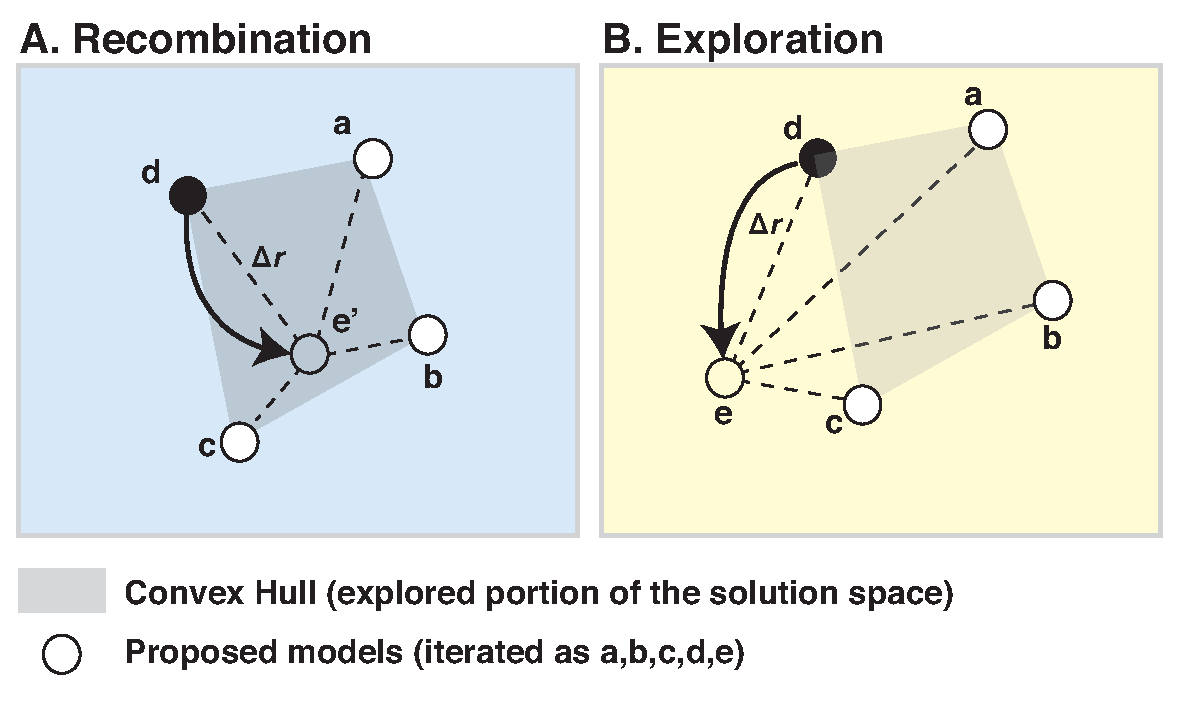
\includegraphics[width=12cm]{figures/figure2.eps}
\caption{\footnotesize{Simplified diagram of exploration and recombination on a plane: {\bf A. Recombination:} iteration {\bf e'} does not incorporate new information. It is a convex combination of all previous proposed solutions (i.e., $\{a,b,c,d\}$).  {\bf B. Exploration:} the average distance between iteration {\bf e} and all previous iterations is larger than half of the maximum distance between any previous proposed solutions. Exploration is not memoryless: {\bf e} is closer to {\bf c} and {\bf d} than {\bf a} and {\bf b}. }}
\label{fig:2}
\end{center}
\end{figure}

Currently, it is poorly understood how cognitive exploration brings new understanding, which is then recombined with previously acquired knowledge, stored in memory (see Figure \ref{fig:2}A). Exploration occurs by leveraging memory (see Figure \ref{fig:2}B). While exploration entails a component of chance (beyond the previous cognitive frontier), recombination can be optimised to find the best possible recombination, which corresponds to the optimal proposed solution (i.e., as close as possible from the true solution) within the cognitive frontier.\\

The experiment conducted at Columbia University Social Science laboratory asked 96 participants to reverse engineer a Bayesian Network with its conditional probabilities and dependencies between nodes. It reveals fine grained mechanisms of how people struggle to balance recombination of mental structures stored in memory with exploration beyond their current cognitive frontier.  Our results suggest that displacement $0.1 < \Delta r < 0.2 $ is particularly beneficial for making progress toward the correct solution. We also find that large displacements seem to require orders of magnitude more ``brain processing" time compared to small displacements. Displacement $0.1 < \Delta r < 0.2 $ is precisely at the inflexion point before waiting times get punishingly long. Yet the degree to which improvements result from strategy and from luck is impossible to parse.

This article is organized as follows. We first report on the experimental results, in particular deviations from a memoryless L\'evy Walks/Flights, such as peculiar returns to previously visited solutions, {\bf anomalous mean square displacement following return and recombination [more work is needed here]}, explorations beyond the cognitive frontier, as well as waiting-time and long-memory processes. We then show how memory, exploration and recombination influence performance. {\bf Building on theoretical consideration in conjunction with observed stylized facts, we test a model of mechanics of cognition in situations in which people tackle hard problems [remains to be done. It may incorporate some Hawkes Processes, but not 100\% sure yet]}. 

\subsection{Experiment}
In our experiment, participants were asked to reverse engineer a multidimensional stochastic process, explicitly expressed in the form of a Bayesian network. They were given 40 minutes, and all changes made were recorded at a 1 second resolution. Participants trying to find the best solution faced a though problem: The {\it simple} process had 3 binary variables, which means that the problem can be thought of as the simultaneous estimation of $(2^3) = 8$ parameters, or the 8 dimensional vector $\mathbf{s}$ with $0 \leqslant s_k  \leqslant 1$ for $k = \{1,...,8\}$ (resp. $k = \{1,..., 16\}$ for the 4 variable {\it complex} stochastic system).


\clearpage

%The cognitive  as well as the evolutionary \cite{radicchi2012evolution} underpinnings of L\'evy walks by humans has been questioned and investigated. The ramifications of L\'evy walks in the mind with foraging / mobility patterns in the physical space: here we question if 
%our mind has been shaped by evolutionary pressure and humans resort to similar strategies. Recent research on online bids \cite{radicchi2012rationality} found similar L\'evy walk patterns even though they appear sup-optimal and even slightly irrational, hence suggesting that L\'evy walks are somehow hard coded in our mind  \cite{radicchi2012evolution}, as humans resort to search strategies, which are no longer fit in the world of information and reasoning with abstract problems, which resolution brings its own incentives and resource rewards in the form of money, recognition, reputation, and pleasure \cite{rewards_modern_societies}.\\

%Here, considering humans facing a hard problem -- typically a unique solution in a complicated problem space -- mental search patterns may be inherited from similar L\'evy walks/flights foraging and mobility patterns �\cite{rhodes2007human,radicchi2012rationality,radicchi2012evolution}.\\

%However, these findings were based on specific cases, involving a specific type of auctions \cite{baronchelli2013levy}. It is also considered that the strategy used is L\'evy walks/flights because it is optimal. However, only truly random L\'evy walks/flights are optimal. True randomness is equivalent to a memoryless process, which would allow exploring the solution space with no consideration of previous knowledge. (a evolutionary theory framework is used to rationalise their findings).\\

%Searching for (or tending/optimizing to) a unique solution involves try and fail, and progressive learning. One may think of an evolutionary process (e.g., ``Animals explore the environment mainly for searching food resources, and it is therefore plausible to ascribe the optimality of their search strategies to a selective evolutionary process."  \cite{radicchi2012evolution}), a Markov process \cite{}, or a process with long range memory, in which candidate solutions explored in the past are reused, and recombined with more recent explored solutions. Finally, some new solutions are truly explored out of the currently explored solution envelop.\\
 
% \subsection{Experiment}
%In our experiment, participants were asked to reverse engineer a Bayesian network. They were given 40 minutes, and all changes made were recorded at a 1 second resolution. Participants trying to reverse the best solution face a though problem: The {\it simple} Bayesian network has 3 nodes, and is defined by a 8-parameters vector $\mathbf{s}$ with $0 \leqslant s_k  \leqslant 1$ for $k = \{1,...,8\}$ (resp. $k = \{1,..., 16\}$ for the 4 node {\it complex} Bayesian network). 
 
 
%\subsection{L\'evy Flight / CTRW}
%We first find that the search process follows a L\'evy flight process with waiting times between moves are random variables, which can be accounted together as a continuous time random walk. Both the distributions of displacement (Figure \ref{fig:pdfs}A ) and waiting times (Figure \ref{fig:pdfs}B ) exhibit power law distributions  (Probability density function of displacement $pdf(\Delta r) = \Delta r^{-\alpha -1}$ with $\alpha = 0.40(5)$. {\bf B.} Probability density function of waiting time $\Delta t$ $pdf(\Delta t) = \Delta t^{-\beta -1}$ with 2 regimes : $\beta_{\Delta t < 125} = 0.38(4)$ and $\beta_{\Delta t > 125} = 1.59(5)$. Distributions of $\Delta r$ and $\Delta t$ are equivalent for the simple and complex treatments.){\bf Problem :} Such CTRW process should normally follow ballistic diffusion characterized by mean square displacement (MSD) and diffusion $\sim t^{\mu}$ with  $\mu_{Levy} = 1$ or super-diffusion $\mu_{CTRW} = \beta$ \cite{21,23}). Here, however, mean square displacement (MSD) decays as $\sim t^{\mu}$ with $\mu_{simple} =-0.23(2)$ and $\mu_{complex} =- 0.26(1)$ showing a slow convergence. 

 
 %Here, we document how such frustrating and somewhat irrational situations may stem from evolutionary homology \cite{evolutionary_homology}, that is mental search properties may share conserved neural substrates with similar neuro-molecular processes guiding spatial search in animals and modulating the control of human attention \cite{hills2006animal}. We show that search strategies inherited from food \cite{food_foraging} and resource \cite{resource_foraging} foraging lead to a form of ``hard-wired bounded rationality" when tackling hard problems.\\

\subsection{L\'evy Flight / CTRW}
We first find that the search process approximately follows a continuous time L\'evy flight process, where waiting times between moves are random variables.  Both the distributions of displacement (Figure \ref{fig:pdfs}A ) and waiting times (Figure \ref{fig:pdfs}B ) are best described by power law distributions  (Probability density function of displacement $pdf(\Delta r) = \Delta r^{-\alpha -1}$ with $\alpha = 0.40(5)$.  Note that this is NOT a L\'evy flight (for which $\alpha$ would have to be between 1 and 3.  {\bf B.} Probability density function of waiting time $\Delta t$ $pdf(\Delta t) = \Delta t^{-\beta -1}$ with 2 regimes : $\beta_{\Delta t < 125} = 0.38(4)$ and $\beta_{\Delta t > 125} = 1.59(5)$. Distributions of $\Delta r$ and $\Delta t$ are equivalent for the simple and complex treatments.)

{\bf Problem :} Such CTRW process should normally follow ballistic diffusion characterized by mean square displacement (MSD) and diffusion $\sim t^{\mu}$ with  $\mu_{Levy} = 1$ \
or super-diffusion $\mu_{CTRW} = \beta$ \cite{21,23}). Here, however, mean square displacement (MSD) decays as $\sim t^{\mu}$ with $\mu_{simple} =-0.23(2)$ and $\mu_{complex} =-\
 0.26(1)$ showing a much slower convergence than would be expected.





